\section{Tutorial A10.2}

\begin{problem}
    Is the following true or false in general?

    \begin{enumerate}
        \item $\abs{w^2} = \abs{w}^2$
        \item $\abs{z + 2w} = \abs{z} + \abs{2w}$
    \end{enumerate}
\end{problem}
\begin{solution}
    \begin{ppart}
        Let $w = r\e^{\i\t}$, where $r, \t \in \RR$. Note that $\abs{\e^{\i\t}} = \abs{\e^{2\i\t}} = 1$. \[\abs{w^2} = \abs{r^2 \e^{2\i\t}} = r^2 \abs{\e^{2\i\t}} = r^2 = r^2 \abs{\e^{\i\t}}^2 = \abs{r\e^{\i\t}}^2 = \abs{w}^2.\] The statement is hence true in general.
    \end{ppart}
    \begin{ppart}
        Take $z = 1$ and $w = -1$. \[\abs{z + 2w} = \abs{1 - 2} = 1 \neq 3 = \abs{1} + \abs{2(-1)} = \abs{z} + \abs{2w}.\] The statement is hence false in general.
    \end{ppart}
\end{solution}

\begin{problem}
    Express the following complex numbers $z$ in polar form $r(\cos\t + \i\sin\t)$ with exact values.

    \begin{enumerate}
        \item $z = 2-2\i$
        \item $z = -1 + \i\sqrt3$
        \item $z = -5\i$
        \item $z = -2\sqrt3 - 2\i$
    \end{enumerate}
\end{problem}
\begin{solution}
    \begin{ppart}
        \begin{center}\tikzsetnextfilename{63}
            \begin{tikzpicture}[trim axis left, trim axis right]
                \begin{axis}[
                    domain = 0:10,
                    samples = 101,
                    axis y line=middle,
                    axis x line=middle,
                    xtick = {2},
                    ytick = {-2},
                    yticklabels = {$-2\i$},
                    xmax=3,
                    xmin=-1,
                    ymin=-3,
                    ymax=1,
                    xlabel = {$\Re$},
                    ylabel = {$\Im$},
                    legend cell align={left},
                    legend pos=outer north east,
                    after end axis/.code={
                        \path (axis cs:0,0) 
                            node [anchor=north east] {$O$};
                        }
                    ]
        
                    \coordinate (R) at (10,0);
                    \coordinate[label=below:$Z(z)$] (Z) at (2, -2);
                    \coordinate (O) at (0, 0);
            
                    \draw (O) -- (Z);
            
                    \fill (Z) circle[radius=2.5pt];
                    \draw pic [draw, angle radius=12mm, "$\t$"] {angle = Z--O--R};
                \end{axis}
            \end{tikzpicture}
        \end{center}

        We have $r^2 = 2^2 + (-2)^2 \implies r = 2\sqrt2$ and $\tan \t = -2/2 \implies \t = -\pi/4$. Hence, $2 - 2\i = 2\sqrt2 \bs{\cos{-\frac\pi4} + \i\sin{-\frac\pi4}}$.
    \end{ppart}
    \begin{ppart}
        \begin{center}\tikzsetnextfilename{64}
            \begin{tikzpicture}[trim axis left, trim axis right]
                \begin{axis}[
                    domain = 0:10,
                    samples = 101,
                    axis y line=middle,
                    axis x line=middle,
                    xtick = {-1},
                    ytick = {sqrt(3)},
                    yticklabels = {$\sqrt3 \i$},
                    xmax=1,
                    xmin=-1.5,
                    ymin=-0.5,
                    ymax=3,
                    xlabel = {$\Re$},
                    ylabel = {$\Im$},
                    legend cell align={left},
                    legend pos=outer north east,
                    after end axis/.code={
                        \path (axis cs:0,0) 
                            node [anchor=north east] {$O$};
                        }
                    ]
        
                    \coordinate (R) at (10,0);
                    \coordinate[label=above:$Z(z)$] (Z) at (-1, 1.73);
                    \coordinate (O) at (0, 0);
            
                    \draw (O) -- (Z);
            
                    \fill (Z) circle[radius=2.5pt];
                    \draw pic [draw, angle radius=12mm, "$\t$"] {angle = R--O--Z};
                \end{axis}
            \end{tikzpicture}
        \end{center}

        We have $r^2 = (-1)^2 + (\sqrt3)^2 \implies r = 2$ and $\tan t = \sqrt{3}/(-1) \implies \t = 2\pi/3$. Hence, $-1 + \sqrt3 \i = 2 \bs{\cos{\frac{2\pi}3} + \i\sin{\frac{2\pi}3}}$.
    \end{ppart}
    \begin{ppart}
        \begin{center}\tikzsetnextfilename{65}
            \begin{tikzpicture}[trim axis left, trim axis right]
                \begin{axis}[
                    domain = 0:10,
                    samples = 101,
                    axis y line=middle,
                    axis x line=middle,
                    xtick = \empty,
                    ytick = {-5},
                    yticklabels = {$-5\i$},
                    xmax=1,
                    xmin=-1,
                    ymin=-6,
                    ymax=1,
                    xlabel = {$\Re$},
                    ylabel = {$\Im$},
                    legend cell align={left},
                    legend pos=outer north east,
                    after end axis/.code={
                        \path (axis cs:0,0) 
                            node [anchor=north east] {$O$};
                        }
                    ]
        
                    \coordinate (R) at (10,0);
                    \coordinate[label=right:$Z(z)$] (Z) at (0, -5);
                    \coordinate (O) at (0, 0);
            
                    \draw (O) -- (Z);
            
                    \fill (Z) circle[radius=2.5pt];
                    \draw pic [draw, angle radius=6mm, "$\t$"] {right angle = Z--O--R};
                \end{axis}
            \end{tikzpicture}
        \end{center}

        We have $r = 5$ and $\t = -\pi/2$. Hence, $-5\i = 5\bs{\cos{-\frac\pi2} + \i\sin{-\frac\pi2}}$.
    \end{ppart}
    \begin{ppart}
        \begin{center}\tikzsetnextfilename{66}
            \begin{tikzpicture}[trim axis left, trim axis right]
                \begin{axis}[
                    domain = 0:10,
                    samples = 101,
                    axis y line=middle,
                    axis x line=middle,
                    xtick = {-3.46},
                    ytick = {-2},
                    xticklabels = {$-2\sqrt3$},
                    yticklabels = {$-2\i$},
                    xmax=1.5,
                    xmin=-4,
                    ymin=-3,
                    ymax=1,
                    xlabel = {$\Re$},
                    ylabel = {$\Im$},
                    legend cell align={left},
                    legend pos=outer north east,
                    after end axis/.code={
                        \path (axis cs:0,0) 
                            node [anchor=south east] {$O$};
                        }
                    ]
        
                    \coordinate (R) at (10,0);
                    \coordinate[label=above:$Z(z)$] (Z) at (-3.46, -2);
                    \coordinate (O) at (0, 0);
            
                    \draw (O) -- (Z);
            
                    \fill (Z) circle[radius=2.5pt];
                    \draw pic [draw, angle radius=12mm, "$\t$"] {angle = Z--O--R};
                \end{axis}
            \end{tikzpicture}
        \end{center}

        We have $r^2 = (-2\sqrt3)^2 + (-2)^2 \implies r = 4$ and $\tan t = -2/(-2\sqrt3) \implies \t = -5\pi/6$. Hence, $-2\sqrt3 - 2\i = 4\bs{\cos{-\frac{5\pi}6} + \i\sin{-\frac{5\pi}6}}$.
    \end{ppart}
\end{solution}

\begin{problem}
    Express the following complex numbers $z$ in exponential form $r\e^{\i\t}$.

    \begin{enumerate}
        \item $z = -1 + \frac2{13}\i$
        \item $z = \cos 50\deg - \i\sin 50\deg$
    \end{enumerate}
\end{problem}
\begin{solution}
    \begin{ppart}
        \begin{center}\tikzsetnextfilename{67}
            \begin{tikzpicture}[trim axis left, trim axis right]
                \begin{axis}[
                    domain = 0:10,
                    samples = 101,
                    axis y line=middle,
                    axis x line=middle,
                    xtick = {-1},
                    ytick = {2/13},
                    yticklabels = {$\frac2{13}\i$},
                    xmax=1,
                    xmin=-2,
                    ymin=-0.1,
                    ymax=0.2,
                    xlabel = {$\Re$},
                    ylabel = {$\Im$},
                    legend cell align={left},
                    legend pos=outer north east,
                    after end axis/.code={
                        \path (axis cs:0,0) 
                            node [anchor=north east] {$O$};
                        }
                    ]
        
                    \coordinate (R) at (10,0);
                    \coordinate[label=above:$Z(z)$] (Z) at (-1, 2/13);
                    \coordinate (O) at (0, 0);
            
                    \draw (O) -- (Z);
            
                    \fill (Z) circle[radius=2.5pt];
                    \draw pic [draw, angle radius=12mm, "$\t$"] {angle = R--O--Z};
                \end{axis}
            \end{tikzpicture}
        \end{center}

        We have $r^2 = (-1)^2 + \bp{\frac2{13}}^2 \implies r = 1.01 \tosf{3}$ and $\tan t = \frac{2/13}{-1} \implies \t = 2.99 \tosf{3}$. Hence, $-1 + \frac2{13}\i = 1.01\e^{2.99\i}$.
    \end{ppart}
    \begin{ppart}
        We have $r = 1$ and $\t = -50\deg = -\frac5{18}\pi$. Hence, $\cos 50 \deg + i \sin 50 \deg = \e^{-\i\frac5{18}\pi}$.
    \end{ppart}
\end{solution}

\begin{problem}
    Express the following complex numbers $z$ in Cartesian form.

    \begin{enumerate}
        \item $z = 7\e^{1 - 5\i}$
        \item $z = 6\bp{\cos \frac\pi8 - \i\sin\frac\pi8}$
    \end{enumerate}
\end{problem}
\begin{solution}
    \begin{ppart}
        We have \[z = 7\e^{1-5\i} = 7\e \cdot \e^{-5\i} = 7\e \bs{\cos{-5} + \i\sin{-5}} = 5.40 + 18.2\i \tosf{3}.\]
    \end{ppart}
    \begin{ppart}
        We have \[z = 6\bp{\cos \frac\pi8 - \i\sin\frac\pi8} = 5.54 - 2.30\i \tosf{3}.\]
    \end{ppart}
\end{solution}

\clearpage
\begin{problem}
    Given that $z = \sqrt3 - \i$, find the exact modulus and argument of $z$. Hence, find the exact modulus and argument of $1/z^2$ and $z^{10}$.
\end{problem}
\begin{solution}
    \begin{center}\tikzsetnextfilename{68}
        \begin{tikzpicture}[trim axis left, trim axis right]
            \begin{axis}[
                domain = 0:10,
                samples = 101,
                axis y line=middle,
                axis x line=middle,
                xtick = {sqrt(3)},
                xticklabels={$\sqrt3$},
                ytick = {-1},
                yticklabels = {$-\i$},
                xmax=2,
                xmin=-0.5,
                ymin=-1.5,
                ymax=0.5,
                xlabel = {$\Re$},
                ylabel = {$\Im$},
                legend cell align={left},
                legend pos=outer north east,
                after end axis/.code={
                    \path (axis cs:0,0) 
                        node [anchor=north east] {$O$};
                    }
                ]
    
                \coordinate (R) at (10,0);
                \coordinate[label=below:$Z(z)$] (Z) at (1.73, -1);
                \coordinate (O) at (0, 0);
        
                \draw (O) -- (Z);
        
                \fill (Z) circle[radius=2.5pt];
                \draw pic [draw, angle radius=12mm, "$\t$"] {angle = Z--O--R};
            \end{axis}
        \end{tikzpicture}
    \end{center}

    We have $r^2 = (\sqrt3)^2 + (-1)^2 \implies r = 2$ and $\tan \t = -1/\sqrt3 \implies \t = -\pi/6$. Hence, $\abs{z} = 2$ and $\arg z = -\pi/6$.

    Note that $\abs{1/z^2} = \abs{z}^{-2} = 1/4$. Also, $\arg{1/z^2} = -2 \arg z = \pi/3$.

    Note that$\abs{z^{10}} = \abs{z}^10 = 1024$. Also, $\arg z^{10} = 10 \arg z = -5\pi/3 \equiv \pi/3$.
\end{solution}

\begin{problem}
    If $\arg{z - 1/2} = \pi/5$, determine $\arg{2z - 1}$.
\end{problem}
\begin{solution}
    \[\arg{2z - 1} = \arg{\frac12 \bs{z - \frac12}} = \arg{z - \frac12} = \frac\pi5.\]
\end{solution}

\begin{problem}
    In an Argand diagram, points $P$ and $Q$ represent the complex numbers $z = 1 + \i$ and $w = 1 + 2\i$ respectively, and $O$ is the origin.

    \begin{enumerate}
        \item Mark on the Argand diagram the points $P$ and $Q$, and the points $R$ and $S$ which represent $z + w$ and $iw$ respectively.
        \item What is the geometrical shape of $OPRQ$?
        \item State the angle $SOP$.
    \end{enumerate}
\end{problem}
\begin{solution}
    \begin{ppart}
        \begin{center}\tikzsetnextfilename{69}
            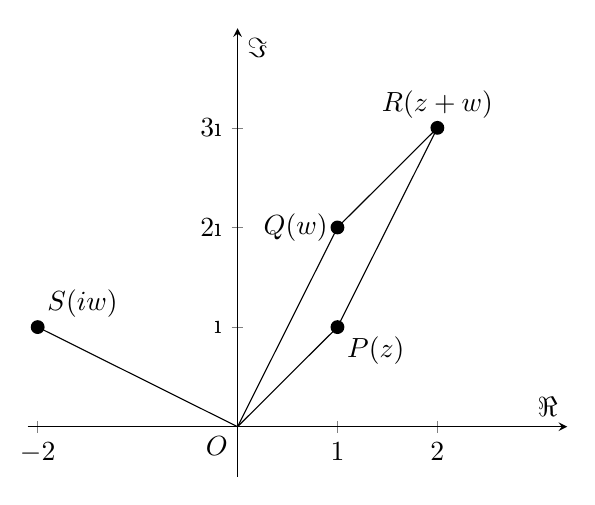
\begin{tikzpicture}[trim axis left, trim axis right]
                \begin{axis}[
                    domain = 0:10,
                    samples = 101,
                    axis y line=middle,
                    axis x line=middle,
                    xtick = {-2, 1, 2},
                    ytick = {1, 2, 3},
                    yticklabels = {$\i$, $2\i$, $3\i$},
                    xmax=3.3,
                    xmin=-2.1,
                    ymin=-0.5,
                    ymax=4,
                    xlabel = {$\Re$},
                    ylabel = {$\Im$},
                    legend cell align={left},
                    legend pos=outer north east,
                    after end axis/.code={
                        \path (axis cs:0,0) 
                            node [anchor=north east] {$O$};
                        }
                    ]
        
                    \coordinate (R) at (10,0);
                    \coordinate[label=below right:$P(z)$] (P) at (1, 1);
                    \coordinate[label=left:$Q(w)$] (Q) at (1, 2);
                    \coordinate[label=above:$R(z+w)$] (R) at (2, 3);
                    \coordinate[label=above right:$S(iw)$] (S) at (-2, 1);
                    \coordinate (O) at (0, 0);
            
                    \draw (O) -- (P);
                    \draw (O) -- (Q);
                    \draw (Q) -- (R);
                    \draw (P) -- (R);
                    \draw (O) -- (S);
            
                    \fill (P) circle[radius=2.5pt];
                    \fill (Q) circle[radius=2.5pt];
                    \fill (R) circle[radius=2.5pt];
                    \fill (S) circle[radius=2.5pt];
                \end{axis}
            \end{tikzpicture}
        \end{center}
    \end{ppart}
    \begin{ppart}
        $OPRQ$ is a parallelogram.
    \end{ppart}
    \begin{ppart}
        $\angle SOP = \pi/2$.
    \end{ppart}
\end{solution}

\begin{problem}
    $B$ and $D$ are points in the Argand diagram representing the complex numbers $1 + 5\i$ and $5 + 3\i$ respectively. Given that $BD$ is a diagonal of the square $ABCD$, calculate the complex numbers represented by $A$ and $C$.
\end{problem}
\begin{solution}
    \begin{center}\tikzsetnextfilename{70}
        \begin{tikzpicture}[trim axis left, trim axis right]
            \begin{axis}[
                domain = 0:10,
                samples = 101,
                axis y line=middle,
                axis x line=middle,
                xtick = {1, 5},
                ytick = {3, 5},
                yticklabels = {$3\i$, $5\i$},
                xmax=9,
                xmin=-1,
                ymin=-1,
                ymax=8,
                xlabel = {$\Re$},
                ylabel = {$\Im$},
                legend cell align={left},
                legend pos=outer north east,
                after end axis/.code={
                    \path (axis cs:0,0) 
                        node [anchor=north east] {$O$};
                    }
                ]
    
                \coordinate (R) at (10,0);
                \coordinate[label=below:$A$] (A) at (2, 2);
                \coordinate[label=left:$B$] (B) at (1, 5);
                \coordinate[label=above:$C$] (C) at (4, 6);
                \coordinate[label=right:$D$] (D) at (5, 3);
                \coordinate (O) at (0, 0);

                \draw (A) -- (B);
                \draw (B) -- (C);
                \draw (C) -- (D);
                \draw (D) -- (A);
                    
                \fill (A) circle[radius=2.5pt];
                \fill (B) circle[radius=2.5pt];
                \fill (C) circle[radius=2.5pt];
                \fill (D) circle[radius=2.5pt];
            \end{axis}
        \end{tikzpicture}
    \end{center}

    Let $A(x + \i y)$. Since $AB \perp AD$, we have $b - a = \i(d - a)$. Thus, \[(1 + 5\i) - (x + \i y) = i\bs{(5 + 3\i) - (x + \i y)},\] which simplifies to \[(x + y) + (y - x)\i = 4.\] Comparing real and imaginary parts, we obtain $x = y = 2$. Hence, $A(2 + 2\i)$.

    Let $C(u + \i v)$. Since $CB \perp CD$, we have $d - c = \i(b - c)$. Thus, \[(5 + 3\i) - (u + \i v) = \i\bs{(1 + 5\i) - (u + \i v)},\] which simplifies to \[(u + v) + (v - u)\i = 10 + 2\i.\] Comparing real and imaginary parts, we obtain $u = 4$ and $v = 6$. Hence, $C(4 + 6\i)$.
\end{solution}

\begin{problem}
    \begin{enumerate}
        \item Given that $u = 2\bp{\cos\frac\pi6 + \i\sin\frac\pi6}$ and $w = 4\bp{\cos\frac\pi3 - \i\sin\frac\pi3}$, find the modulus and argument of $u\conj/w^3$ in exact form.
        \item Let $z$ be the complex number $-1 + \i\sqrt3$. Find the value of the real number $a$ such that $\arg{z^2 + az} = -\pi/2$.
    \end{enumerate}
\end{problem}
\begin{solution}
    \begin{ppart}
        Note that $\abs{u} = 2$, $\arg u = \pi/6$, $\abs{w} = 4$ and $\arg w = -\pi/3$. Hence, \[\abs{\frac{u\conj}{w^3}} = \frac{\abs{u\conj}}{\abs{w^3}} = \frac{\abs{u}}{\abs{w}^3} = \frac{2}{4^3} = \frac1{32}\] and \[\arg \frac{u\conj}{w^3} = \arg u\conj - \arg w^3 = -\arg u - 3\arg w = -\frac\pi6 - 3 \bp{-\frac\pi3} = \frac56 \pi.\]
    \end{ppart}
    \begin{ppart}
        Since $\arg{z^2 + az} = -\pi/2$, we have that $z^2 + az$ is purely imaginary, with a negative imaginary part. Since \[z^2 + az = \bp{-1 + \i\sqrt3}^2 + a\bp{-1 + \i \sqrt3} = \bp{-2 -2\sqrt3 \i} + a\bp{-1 + \i\sqrt3}.\] Hence, \[\Re{z^2 + az} = 0 \implies -2 -a = 0 \implies a = -2.\]
    \end{ppart}
\end{solution}

\begin{problem}
    The complex number $w$ has modulus $r$ and argument $\t$, where $0 < \t < \pi/2$, and $w\conj$ denotes the conjugate of $w$. State the modulus and argument of $p$, where $p = w/w\conj$. Given that $p^5$ is real and positive, find the possible values of $\t$.
\end{problem}
\begin{solution}
    Clearly, $\abs{p} = 1$ and $\arg p = 2\t$.

    Since $p^5$ is real and positive, we have $\arg p^5 = 2\pi n$, where $n \in \ZZ$. Thus, $\arg p = 2\pi n/5 = 2\t \implies \t =\pi n/5$. Since $0 < \t < \pi/2$, the possible values of $\t$ are $\pi/5$ and $2\pi/5$.
\end{solution}

\begin{problem}
    The complex number $w$ has modulus $\sqrt2$ and argument $-3\pi/4$, and the complex number $z$ has modulus 2 and argument $-\pi/3$. Find the modulus and argument of $wz$, giving each answer exactly.

    By first expressing $w$ and $z$ in the form $x + \i y$, find the exact real and imaginary parts of $wz$.

    Hence, show that $\sin \frac\pi{12} = \frac{\sqrt3 - 1}{2\sqrt2}$.
\end{problem}
\begin{solution}
    Note that \[\abs{wz} = \abs{w} \abs{z} = 2\sqrt2\] and \[\arg{wz} = \arg w + \arg z = - \frac34 \pi - \frac13 \pi = -\frac{13}{12}\pi \equiv \frac{11}{12} \pi.\]

    Also, \[w = \sqrt2 \bs{\cos{-\frac34 \pi} + \i\sin{-\frac34 \pi}} = \sqrt2 \bp{-\frac1{\sqrt2} - \frac1{\sqrt2} \i} = -1-\i\] and \[z = 2\bs{\cos{-\frac\pi3} + \i\sin{-\frac\pi3}} = 2\bp{\frac12 - \frac{\sqrt3}{2} \i} = 1 - \sqrt3 \i.\] Hence, \[wz = (-1 - \i)(1 - \sqrt3 \i) = (-1 + \sqrt3 -\i - \sqrt3) = (-1 - \sqrt3) + (\sqrt3 - 1)\i,\] whence $\Re{wz} = -1 - \sqrt3$ and $\Im{wz} = \sqrt3 - 1$.

    From the first part, we have that $wz = 2\sqrt2 \bs{\cos{\frac{11}{12} \pi} + \i\sin{\frac{11}{12} \pi}}$. Thus, $\Im{wz} = 2\sqrt{2} \sin{\frac{11}{12} \pi} = 2\sqrt2 \sin \frac\pi{12}$. Equating the result for $\Im{wz}$ found in the second part, we have \[2\sqrt2 \sin \frac\pi{12} = \sqrt3 - 1 \implies \sin \frac{\pi}{12} = \frac{\sqrt3 - 1}{2\sqrt2}.\]
\end{solution}

\clearpage
\begin{problem}
    Given that $\frac{5 + z}{5 - z} = \e^{\i\t}$, show that $z$ can be written as $5\i\tan\frac\t2$.
\end{problem}
\begin{solution}
    Note that \[\frac{5 + z}{5 - z} = \e^{\i\t} \implies 5 + z = \e^{\i\t} (5-z) \implies z + \e^{\i\t}z = 5\e^{\i\t} - 5 \implies z = 5 \bp{\frac{\e^{\i\t} - 1}{\e^{\i\t} + 1}}.\] Hence, \[z = 5\bp{\frac{\e^{\i\t} - 1}{\e^{\i\t} + 1}} = 5\bp{\frac{\e^{\i\t/2} - \e^{-\i\t/2}}{\e^{\i\t/2} + \e^{-\i\t/2}}} = 5\bp{\frac{2\i \sin{\t/2}}{2\cos{\t/2}}} = 5\i\tan \frac\t2.\]
\end{solution}

\begin{problem}
    The polynomial $P(z)$ has real coefficients. The equation $P(z) = 0$ has a root $r\e^{\i\t}$, where $r > 0$ and $0 < \t < \pi$.

    \begin{enumerate}
        \item Write down a second root in terms of $r$ and $\t$, and hence show that a quadratic factor of $P(z)$ is $z^2 - 2rz\cos\t + r^2$.
        \item Given that 3 roots of the equation $z^6 = -64$ are $2\e^{\i \frac\pi6}$, $2\e^{\i\frac\pi2}$ and $2\e^{-\i\frac{5\pi}6}$, express $z^6 + 64$ as a product of three quadratic factors with real coefficients, giving each factor in non-trigonometric form.
        \item Represent all roots of $z^6 = -64$ on an Argand diagram and interpret the geometrical shape formed by joining the roots.
    \end{enumerate}
\end{problem}
\begin{solution}
    \begin{ppart}
        Since $P(z)$ has real coefficients, by the conjugate root theorem, $\bp{r\e^{\i\t}}\conj = r\e^{-\i\t}$ is also a root of $P(z)$. By the factor theorem, a quadratic factor of $P(z)$ is \[(z - r\e^{\i\t})(z - r\e^{-\i\t}) = z^2 -rz(\e^{\i\t} + \e^{-\i\t}) + r^2\e^{\i\t}\e^{-\i\t} = z^2 - 2rz\cos\t + r^2.\]
    \end{ppart}
    \begin{ppart}
        Let $r_1 = r_2 = r_3 = 2$ and $\t_1 = \pi/6$, $\t_2 = \pi/2$ and $\t_3 = -5\pi/6$.
        \begin{align*}
            z^6 + 64 &= \bp{z^2 - 2r_1z\cos\t_1 + r_1^2}\bp{z^2 - 2r_2z\cos\t_2 + r_2^2}\bp{z^2 - 2r_3z\cos\t_3 + r_3^2}\\
            &= \bp{z^2 - 4z\cos{\frac\pi6} + 4}\bp{z^2 - 4z\cos{\frac\pi2} + 4} \bp{z^2 - 4z\cos{-\frac56 \pi} + 4}\\
            &= \bp{z^2 - 2\sqrt3 z + 4}\bp{z^2 + 4} \bp{z^2 + 2\sqrt3 z + 4}
        \end{align*}
    \end{ppart}
    \begin{ppart}
        \begin{center}\tikzsetnextfilename{71}
            \begin{tikzpicture}[trim axis left, trim axis right]
                \begin{axis}[
                    domain = 0:10,
                    samples = 101,
                    axis y line=middle,
                    axis x line=middle,
                    xtick = \empty,
                    ytick = \empty,
                    xmax=3.3,
                    xmin=-3.3,
                    ymin=-3.3,
                    ymax=3.3,
                    xlabel = {$\Re$},
                    ylabel = {$\Im$},
                    legend cell align={left},
                    legend pos=outer north east,
                    after end axis/.code={
                        \path (axis cs:0,0) 
                            node [anchor=north east] {$O$};
                        }
                    ]
        
                    \coordinate (R) at (10,0);
                    \coordinate[label=right:$Z_1$] (Z1) at (1.73, 1);
                    \coordinate[label=above right:$Z_2$] (Z2) at (0, 2);
                    \coordinate[label=left:$Z_3$] (Z3) at (-1.73, 1);
                    \coordinate[label=left:$Z_4$] (Z4) at (-1.73, -1);
                    \coordinate[label=below right:$Z_5$] (Z5) at (0, -2);
                    \coordinate[label=right:$Z_6$] (Z6) at (1.73, -1);
                    \coordinate (O) at (0, 0);

                    \draw (Z1) -- (Z2);
                    \draw (Z2) -- (Z3);
                    \draw (Z3) -- (Z4);
                    \draw (Z4) -- (Z5);
                    \draw (Z5) -- (Z6);
                    \draw (Z6) -- (Z1);
                            
                    \fill (Z1) circle[radius=2.5pt];
                    \fill (Z2) circle[radius=2.5pt];
                    \fill (Z3) circle[radius=2.5pt];
                    \fill (Z4) circle[radius=2.5pt];
                    \fill (Z5) circle[radius=2.5pt];
                    \fill (Z6) circle[radius=2.5pt];
                \end{axis}
            \end{tikzpicture}
        \end{center}

        The geometrical shape formed is a regular hexagon.
    \end{ppart}
\end{solution}